%  !TeX  root  =  user_guide.tex 

\section{Plugin fTools}\label{sec:ftools}

% when the revision of a section has been finalized, 
% comment out the following line:
% \updatedisclaimer

Il plugin fTools fornisce una risorsa comprensiva delle più 
comuni operazioni GIS basate su vettori, senza la necessità di software addizionale, 
librerie e soluzioni complesse: il plugin mette a disposizione una suite di 
funzioni di analisi veloci e funzionali.

fTools è installato di default nelle nuove versioni di QGIS e, come tutti gli altri plugin, 
può essere disabilitato nel gestore dei plugin (Sezione \ref{sec:managing_plugins}).
Se abilitato, fTools aggiunge il nuovo menu \mainmenuopt{Vettore} all'interfaccia 
di QGIS: questo nuovo menu offre funzioni di ricerca, analisi, geoprocessamento, gestione.

\minisec{Strumenti di fTools}\label{ftool_functions}

Le tabelle da \ref{tab:ftool_analysis} a \ref{tab:fTool_data_management} 
elencano e descrivono brevemente gli strumenti di fTools. 

\begin{table}[ht]\index{Strumenti di Analisi}
\centering
 \begin{tabular}{|m{1cm}|m{3cm}|m{12cm}|}
\hline \multicolumn{3}{|c|}{\textbf{Strumenti di Analisi di fTools}} \\
 \hline \textbf{Icona} & \textbf{Strumento} & \textbf{Azione} \\
 \hline 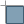
\includegraphics[width=0.7cm]{matrix} & Matrice di distanza &
Misura le distanze tra due layer di punti e fornisce il risultato come a) Matrice 
di distanza lineare, b) Matrice di distanza standard, c) Sintesi matrice di distanza.
Può limitare i calcoli ai 'k' punti più vicini. \\ 
 \hline 
\includegraphics[width=0.7cm]{sum_lines} & Somma lunghezze linee & Calcola
la somma della lunghezza di tutte le linee per ogni poligono di un layer di poligoni. \\
 \hline 
\includegraphics[width=0.7cm]{sum_points} & Punti nel poligono & Calcola il 
numero di punti che ricadono all'interno di ogni poligono di un layer di poligoni. \\
 \hline 
\includegraphics[width=0.7cm]{unique} & Lista valori unici & Elenca i valori 
unici di un campo di un layer vettoriale. \\
 \hline 
\includegraphics[width=0.7cm]{basic_statistics} & Statistiche di base & Calcola 
statistiche di base, es. media, deviazione standard, somma, di un campo di un 
layer vettoriale. \\ 
 \hline 
\includegraphics[width=0.7cm]{neighbour} & Analisi vicino più prossimo & 
Calcola delle statistiche per valutare il livello di clustering in un layer vettoriale 
di punti. \\
 \hline 
\includegraphics[width=0.7cm]{mean} & Media coordinata(e) &
Calcola il centro medio (media normale o pesata) di un layer vettoriale o di 
un'insieme di elementi ed in funzione di un campo con ID unico. \\ 
 \hline 
\includegraphics[width=0.7cm]{intersections} & Intersezioni linee &
Calcola l'intersezione tra linee e restituisce il risultato in uno shapefile di punti. \\
 \hline
\end{tabular}
\caption{fTools - Strumenti di Analisi}\label{tab:ftool_analysis}
\end{table}

\begin{table}[ht]\index{Strumenti di Ricerca}
\centering
 \begin{tabular}{|m{1cm}|m{3cm}|m{12cm}|}
 \hline \multicolumn{3}{|c|}{\textbf{Strumenti di Ricerca di fTools}} \\
 \hline \textbf{Icona} & \textbf{Strumento} & \textbf{Azione} \\
 \hline 
\includegraphics[width=0.7cm]{random_selection} & Selezione causale & Seleziona 
in maniera casuale 'n' o 'n\%' di elementi. \\
 \hline 
\includegraphics[width=0.7cm]{sub_selection} & Selezione casuale con un sottoinsieme & 
Selezione casuale in un sottoinseme tramite campo ID unico. \\
 \hline 
\includegraphics[width=0.7cm]{random_points} & Punti casuali & Genera punti 
pseudo-random. \\
 \hline 
\includegraphics[width=0.7cm]{regular_points} & Punti regolari & Genera 
una griglia regolare di punti su un'area specifica e la esporta come shapefile di punti. \\
 \hline 
\includegraphics[width=0.7cm]{vector_grid} & Reticolo vettoriale & Genera una griglia 
di linee o di poligoni con spaziatura definita dall'utente. \\
 \hline 
\includegraphics[width=0.7cm]{select_location} & Seleziona per posizione & 
Seleziona elementi in base alla loro posizione relativa ad un altro layer: crea una nuova selezione 
oppure aggiunge/sottrae alla selezione corrente. \\
\hline 
\includegraphics[width=0.7cm]{layer_extent} & Poligono dall'estensione del layer & 
Crea un poligono rettangolare dall'estensione di un layer raster o vettoriale. \\
 \hline
\end{tabular}
\caption{fTools - Strumenti di Ricerca}\label{tab:ftool_research}
\end{table}

\begin{table}[ht]\index{Strumenti di Geoprocessing}
\centering
 \begin{tabular}{|m{1cm}|m{3cm}|m{12cm}|}
 \hline \multicolumn{3}{|c|}{\textbf{Strumenti di Geoprocessing di fTools}} \\
 \hline \textbf{Icona} & \textbf{Strumento} & \textbf{Azione} \\
 \hline 
\includegraphics[width=0.7cm]{convex_hull} & Poligono/i convesso/i & Crea il poligono 
minimo convesso di un layer vettoriale o poligoni minimi convessi sulla base di un campo in input. \\
 \hline 
\includegraphics[width=0.7cm]{buffer} & Buffer & Crea buffer intorno ad un elemento 
in funzione di una distanza impostata o di un campo in input. \\
 \hline 
\includegraphics[width=0.7cm]{intersect} & Intersezione & Sovrappone due layer e 
ne restituisce uno nuovo contenente la superficie di intersezione dei layer di input. \\
 \hline 
\includegraphics[width=0.7cm]{union} & Unione & Sovrappone due layer e 
ne restituisce uno nuovo contenente la superficie totale dei layer di input. \\
 \hline 
\includegraphics[width=0.7cm]{sym_difference} & Differenza simmetrica & 
Sovrappone due layer e ne restituisce uno nuovo contenente la superficie dei layer di input
tranne la loro intersezione. \\

 \hline 
\includegraphics[width=0.7cm]{clip} & Clip & Sovrappone due layer e 
ne restituisce uno nuovo contenente la superficie che interseca il 'clip' layer. \\
 \hline 
\includegraphics[width=0.7cm]{difference} & Differenza & Sovrappone due layer e 
ne restituisce uno nuovo contenente la superficie che non interseca il 'clip' layer. \\
 \hline 
\includegraphics[width=0.7cm]{dissolve} & Dissolvenza & Unisce elementi sulla 
base di un campo in input: gli elementi con lo stesso valore sono combinati in un 
elemento unico. \\
 \hline
\end{tabular}
\caption{fTools - Strumenti di Geoprocessing}\label{tab:ftool_geoprocessing}
\end{table}

\begin{table}[ht]\index{Strumenti di Geometria}
\centering
\begin{tabular}{|m{1cm}|m{3cm}|m{12cm}|}
 \hline \multicolumn{3}{|c|}{\textbf{Strumenti di Geometria di fTools}} \\
 \hline \textbf{Icona} & \textbf{Strumento} & \textbf{Azione} \\
 \hline 
\includegraphics[width=0.7cm]{check_geometry} & Controlla validità geometria & 
Controlla poligoni per verificare la presenza di intersezioni e buchi chiusi e 
risolvere l'ordine dei nodi. \\
 \hline 
\includegraphics[width=0.7cm]{export_geometry} & Estrai/Aggiungi colonne geometriche & 
Aggiunge informazioni sulla geometria a layer di punti (XCOORD, YCOORD), di linee
(LENGTH), di poligoni (AREA, PERIMETER). \\
 \hline 
\includegraphics[width=0.7cm]{centroids} & Centroidi di poligoni & 
Calcola i centroidi per ogni poligono di un layer di input. \\
 \hline 
\includegraphics[width=0.7cm]{delaunay} & Triangolazione di Delaunay & 
Calcola la triangolazione di Delaunay per un layer di punti in input. \\
 \hline  & Poligoni di Voronoi & 
Calcola i poligoni di Voronoi per un layer di punti in input. \\
 \hline 
\includegraphics[width=0.7cm]{simplify} & Semplifica geometrie & 
Generalizza linee e/o poligoni con un algoritmo modificato di Douglas-Peucker. \\
 \hline 
\includegraphics[width=0.7cm]{multi_to_single} & Da parti multiple a parti singole & 
Converte elementi multi-parte in più elementi semplici. Crea linee e poligoni semplici. \\
 \hline 
\includegraphics[width=0.7cm]{single_to_multi} & Da parti singole a parti multiple & 
Unisce più elementi in un elemento multi-parte sulla base di un campo in input. \\
 \hline 
\includegraphics[width=0.7cm]{to_lines} & Da poligoni a linee & Converte 
poligoni in linee, poligoni multip-parte in linee semplici. \\
 \hline 
\includegraphics[width=0.7cm]{to_lines} & Da linee a poligoni & Converte 
linee in poligoni, linee multi-parte in poligoni semplici. \\
 \hline 
\includegraphics[width=0.7cm]{extract_nodes} & Estrai vertici & Estrae 
vertici  da layer di linee e poligoni e restituisce un nuovo layer di punti. \\
 \hline
\end{tabular}
\caption{fTools - Strumenti di Geometria}\label{tab:ftool_geometry}
\end{table}

\begin{table}[ht]\index{Strumenti di Gestione Dati}
\centering
\begin{tabular}{|m{1cm}|m{3cm}|m{12cm}|}
 \hline \multicolumn{3}{|c|}{\textbf{Strumenti di Gestione Dati di fTools}} \\
 \hline \textbf{Icona} & \textbf{Strumento} & \textbf{Azione} \\
 \hline 
\includegraphics[width=0.7cm]{define_projection} & Definisci proiezione in uso & 
Specifica il SR per gli shapefile senza SR associato. \\
 \hline 
\includegraphics[width=0.7cm]{join_location} & Unisci attributi per posizione & 
Aggiunge attributi ad un layer vettoriale sulla base di relazioni spaziali. Attributi di 
un layer vengono aggiunti alla tabella attributi di un altro layer: il risultato è 
salvato come nuovo shapefile. \\
 \hline 
\includegraphics[width=0.7cm]{split_layer} & Dividi vettore & 
Divide il layer di input in più layer separati sulla base di un campo in input. \\
 \hline 
\includegraphics[width=0.7cm]{merge_shapes} & Unisci shapefiles &
Unisce più shapefile in un unico shapefile sulla base del tipo di layer (punti, linee, poligoni). \\
 \hline
\end{tabular}
\caption{fTools - Strumenti di Gestione Dati}\label{tab:fTool_data_management}
\end{table}

\FloatBarrier
